% !TEX program = xelatex
% 电子版默认入口。需要纸质前置页时编译 main-print.tex。
\ifdefined\paperprint
  \documentclass[notoc,bwprint]{cumcmthesis}
\else
  \documentclass[withoutpreface,notoc,bwprint]{cumcmthesis}
\fi

% 按团队排版约定取消中文与英文、数字之间的自动间距。
\xeCJKsetup{CJKecglue=\hskip 0pt}
\DeclareCaptionLabelFormat{cjkcompact}{#1#2}
\captionsetup[figure]{labelformat=cjkcompact}
\captionsetup[table]{labelformat=cjkcompact}

\graphicspath{{../figures/}{figures/}}

\title{地缘冲突下国际油价波动预测、宏观传导与中国政策韧性研究}
\tihao{A}
\baominghao{29}
\schoolname{}
\membera{}
\memberb{}
\memberc{}
\supervisor{指导教师}
\yearinput{2026}
\monthinput{8}
\dayinput{1}

% 写作期提示框；提交前全文搜索并删除所有 \draftnote。
\newcommand{\draftnote}[1]{%
  \par\noindent
  \fcolorbox{gray!55}{gray!7}{%
    \parbox{\dimexpr\linewidth-2\fboxsep-2\fboxrule\relax}{\zihao{-5}\textbf{写作提示：}#1}%
  }\par
}

\begin{document}

\maketitle
\begin{abstract}
国际油价由供需基本面、金融条件和地缘风险共同驱动。为避免混淆预测偏差、事件异常与战争净因果
贡献，本文基于2010年1月至2026年6月多源数据，建立“预测与事件识别--结构冲击传导--政策
反事实--尾部风险优化”框架；前问的冲击与响应核依次进入后问，实现四问贯通。

\textbf{针对问题一，}在78个共同目标月上以扩展窗口比较六类预测器。不变预测基线的1、3、6个月
RMSE分别为0.1408、0.2660和0.3082，均为最低；以2026年2月70.887美元/桶为原点，三期点预测
均为70.887美元/桶。状态匹配事件研究得到$CAR[0,+1]=$\textbf{15.61\%}（经验$p=0.0244$），
航运受阻阶段条件波动率为战前的2.214倍；递归SVAR将3月36.45\%的实际收益中的32.23\%
识别为供给收缩贡献，总结构贡献处于历史98.4\%分位。上述结果表明事件附近存在异常，
但不等同于战争净因果份额。

\textbf{针对问题二，}将186个月的三类SVAR冲击输入局部投影，并以2000次移动块bootstrap构造
95\%联合置信带。一次标准差石油特定风险冲击使人民币原油成本当月上升
\textbf{8.832\%}，联合区间为$[6.888\%,10.776\%]$；PPI、CPI峰值分别为0.762\%、0.247\%，
工业增加值第12个月谷值为$-0.427\%$。后三者联合区间均跨零，故模型支持“成本
先行、物价滞后、工业活动可能承压”的顺序，但\textbf{尚无稳健的总体增长损失证据}。

\textbf{针对问题三，}以燃油分布滞后、面板局部投影和动态反事实评价政策。六国6个月零售燃油
传导率中位数为0.227；中国调价指数代理为0.373，因价格层不同不纳入正式排名。部分识别的临界
缩放系数中位数为0.590，95\%区间为$[0.436,0.834]$。若关闭2026年临时调控，6月PPI、CPI将
分别高2.596\%（$[1.453\%,3.633\%]$）和0.414\%（$[0.199\%,1.088\%]$），工业增加值差额
为$-0.469\%$且区间跨零；物价缓冲同时形成\textbf{1425元/吨延期缺口}。因此现有证据
支持条件情景下的局部物价缓冲，但不足以证明我国总体韧性全面优于对照国。

\textbf{针对问题四，}FHS--GJR--GARCH的20000条路径给出6个月Brent中位数71.76美元/桶、
90\%区间$[37.15,117.90]$美元/桶，期末和路径内曾超过历史95\%阈值的概率分别为5.56\%和9.65\%。
提出的\textbf{SAPR--CVaR三状态自适应调价模型}从1771组规则中筛得119组1\%容差Pareto解，
最终传导率为$(0.30,0.10,0.10)$。在2022年至2026年的49个隔离检验情景中，相对完全传导，
平均宏观损失、95\%尾部损失和调价波动分别\textbf{降低47.70\%、38.79\%和30.28\%}，代价是
平均延期缺口负担增加2.22\%；2000次联合块bootstrap中，相对三种预注册基线保持非支配的
概率为100\%。该“最优”仅限本文注册的规则族、六个月情景库和四目标准则。

\keywords{国际油价\quad{}结构VAR\quad{}局部投影\quad{}政策反事实\quad{}SAPR--CVaR}
\end{abstract}


% 2026 电子提交规范不设置目录。
\section{问题重述与研究目标}

国际原油既是基础能源，也是高度金融化的全球大宗商品。其价格同时受到供需基本面、
库存与美元条件、市场预期以及地缘政治风险影响。地缘冲突发生后，供给中断预期、海运
受阻和风险溢价可能在数个交易日内推高油价与波动率；随后，外部冲击又会通过汇率与
进口成本进入国内成品油、工业品和居民消费价格，并最终作用于工业活动和经济增长。
因此，本题不能只建立单一预测模型，而需把``预测是否准确''、``事件期是否异常''、
``冲击如何传导''和``政策如何缓冲''分别识别后再衔接。

题面未给出``美伊战争''的精确起止日。本文将其操作性定义为：2026年2月28日开始的
中东地区军事行动及其引致的霍尔木兹海峡运输中断，并以6月17日通行恢复谅解备忘录
作为缓和阶段起点。由于2月28日为非交易日，日度事件研究从首个共同交易日
2026年3月2日开始。3月23日和4月7日的中国成品油临时调控属于国内政策事件，
不与外部战争事件合并编码。

据此，将研究任务重述为以下四个相互递进的问题：

\begin{enumerate}
  \item 以Brent现货价为国际油价主指标，在严格的时间滚动评价下预测未来
  1、3、6个月价格；同时利用日度事件研究、描述性自回归基准路径和条件波动模型，
  量化冲突不同阶段的异常价格变化与波动变化。
  \item 将第一问识别的供给、全球总需求和石油特定风险冲击作为统一输入，估计其经
  人民币原油成本、PPI、CPI和工业增加值传导至中国经济的方向、幅度、滞后和不确定性，
  并用季度实际GDP作低频验证。
  \item 对中国及六个主要石油进口国构造可比的燃油价格、CPI和工业活动面板，先量化
  中国是否表现出更强韧性，再通过缓冲变量交互和``关闭2026年临时调控''反事实解释
  政策作用及其延期成本。
  \item 利用题面``包括但不限于''的开放性，进一步研究极端油价的条件尾部概率，并在
  现行成品油调价机制约束上设计状态自适应价格平滑规则，为不同压力状态下的调价决策
  提供可检验方案。
\end{enumerate}

本文统一以2026年6月30日为观测截止日。日度层只承担事件识别和风险模拟，月度层
贯通四问，季度GDP不插值为月度数据。这样的分层使短期市场异常、历史结构冲击、宏观
响应和政策情景各自保持清楚的证据边界。

\section{问题分析与总体思路}

\subsection{问题之间的逻辑关系}

第一问包含预测与识别两个不同任务。油价预测检验模型能否利用截止日前信息降低样本外
误差；事件研究检验冲突发生后是否出现相对历史规律异常的收益与波动。预测残差本身不能
被解释为战争的净因果贡献。进一步地，同样的油价上涨可能源于供给收缩、全球需求扩张或
预防性需求，三者对进口国宏观经济的含义不同。本文因此采用Kilian的结构分解思想
\cite{kilian2009}，把三类结构冲击送入第二问，而将Caldara--Iacoviello地缘政治风险指数
作为预测与事件控制信息\cite{caldara2022}。

第二问回答冲击如何沿``人民币原油成本---生产价格---消费价格与工业活动''传导；第三问
把这一传导框架扩展到七国比较，并在中国官方受管制成品油价格层上构造政策关闭情景；
第四问则把未来油价分布、历史结构冲击压力与政策优化组织为三个不可加总但相互衔接的
证据层。总体路线见图\ref{fig:route}。

\begin{figure}[H]
  \centering
  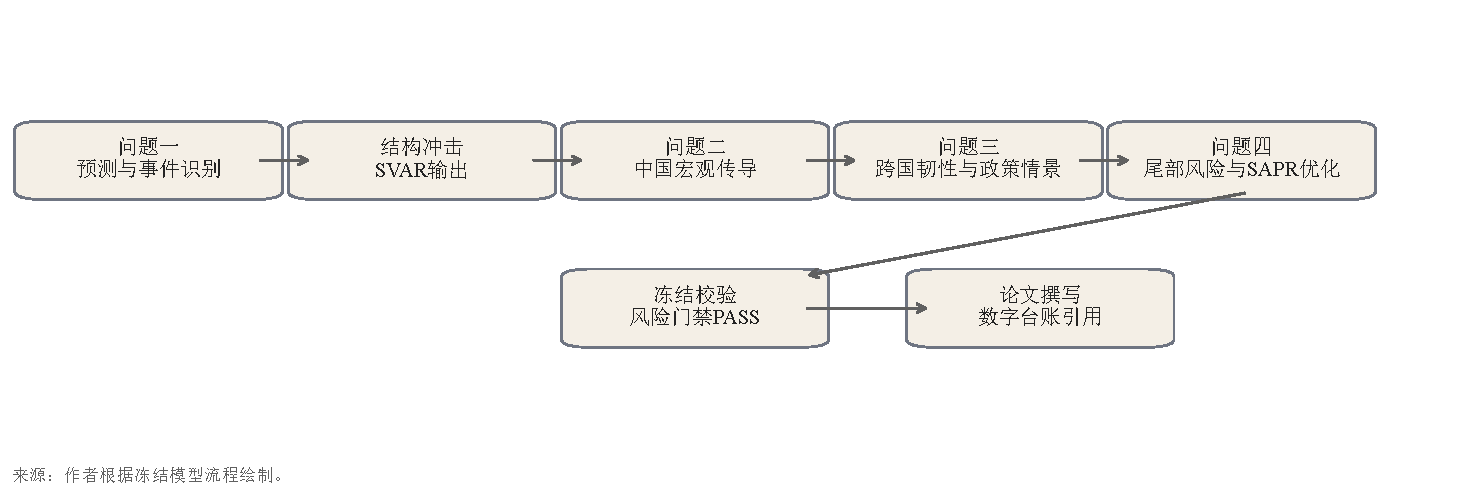
\includegraphics[width=0.92\textwidth]{../figures/paper_route_map.pdf}
  \caption{国际油价冲击研究的总体技术路线}
  \label{fig:route}
\end{figure}

\subsection{数据结构与口径统一}

主样本为2010年1月至2026年6月，共198个月。Brent、WTI、广义美元指数和人民币
汇率由公开日度序列聚合；美国商业原油库存采用月末最后一个已发布周值；GPR使用固定
下载版本的月度指数。中国PPI和规模以上工业增加值来自国家统计局，工业增加值1--2月
合并发布形成的结构性空值原样保留，不作线性插值。人民币原油成本以
``Brent美元价乘人民币兑美元汇率''构造，避免不完整进口单位价值破坏主样本。

跨国部分包含中国、德国、法国、意大利、西班牙、日本和韩国。中国使用受管制汽油标准品
最高零售限价，2013年3月至2026年6月共有160个有效月；欧洲使用含税Euro-super 95，
日本和韩国使用普通汽油全国价格。各币种先与本币Brent配对后取对数变化，从而消除币值
和绝对价格水平差异。整体CPI统一转为同比，工业活动统一使用同比或可比响应。主要公开
数据源与处理见表\ref{tab:data-source}。

\begin{table}[H]
  \centering
  \small
  \caption{核心数据、频率及处理口径}
  \label{tab:data-source}
  \begin{tabularx}{0.98\textwidth}{p{0.19\textwidth}p{0.22\textwidth}p{0.13\textwidth}X}
    \toprule
    数据模块 & 来源 & 原始频率 & 统一处理与用途 \\
    \midrule
    Brent、WTI、汇率 & EIA/FRED\cite{freddata} & 日度 & 交易日事件研究；自然月有效观测均值进入月度模型 \\
    美国商业原油库存 & EIA\cite{eiadata} & 周度 & 月末最后一个已发布周值，防止月内后见信息 \\
    GPR & Caldara--Iacoviello\cite{caldara2022} & 月度 & 使用2026-07-01固定版本，近期值允许后续修订 \\
    中国PPI、IAV、GDP & 国家统计局\cite{nbsdata} & 月/季度 & PPI、IAV进入月度传导；GDP仅作季度验证 \\
    七国CPI、工业活动 & OECD\cite{oecddata} & 月度 & CPI同比与工业活动可比响应；保留方法口径标识 \\
    七国燃油价格 & 各国官方或公开数据中心 & 周/月/事件 & 月均化后与本币Brent对数收益匹配 \\
    中国调价政策 & 国家发展改革委\cite{ndrc2016} & 事件 & 编码机制应调、实际调价及累计未调价差额 \\
    \bottomrule
  \end{tabularx}
\end{table}

所有预测均按时间扩展窗口估计，外生变量至少滞后一期；完整月均值只在月末以后使用。
所有模型共用随机种子20260730。关键结果保存为冻结数值，正文只按预先规定精度展示，
不从图中目测或事后改变口径。

\subsection{四问求解策略}

问题一以no-change为可用基线，将ARIMA、SARIMAX、ETS、Theta和等权组合置于相同
滚动回测中；冲突影响使用交易日累计异常收益、匹配周末安慰剂和GJR--GARCH条件波动率，
历史三类结构冲击则由递归VAR给出。问题二对每个宏观结果变量估计局部投影，并以
ARDL、冲击正负拆分和季度GDP验证稳健性。问题三先做分国分布滞后传导率，再做含国家
与年月固定效应的相对中国面板局部投影，最后关闭临时调控构造价格及宏观反事实。问题四
使用FHS--GJR--GARCH生成条件尾部分布，并在开发样本上枚举三档传导规则，通过四目标
Pareto前沿选择膝点，在隔离检验样本和2026冲击上验证。

\section{模型假设}

\begin{enumerate}
  \item \textbf{实时信息集假设。}预测原点之后的观测不进入估计、调参或阈值选择；统计序列按实际
  发布滞后截断。固定下载版本可能被后续修订，但不回填未来信息。
  \item \textbf{交易日映射假设。}非交易日事件映射到其后首个共同交易日。短窗口仍可能叠加其他
  新闻，故CAR只解释为事件相关异常；常规正态区间为描述性结果，正式显著性依赖状态匹配安慰剂。
  \item \textbf{递归结构识别假设。}月内全球供给响应最慢，全球真实活动可当期响应供给，实际油价
  可当期响应前两者。递归排序为“供给增长---全球真实活动---实际Brent收益”，并用替代排序探针
  检验结论依赖性。
  \item \textbf{局部动态假设。}主要宏观响应在12个月内体现；PPI、CPI、IAV和原油成本的被解释量
  为未来水平，汇率为相对冲击前基期的累计对数变化。移动块bootstrap保留月度序列依赖。
  \item \textbf{跨国可比边界。}六个对照国的官方零售燃油对数收益可以比较；中国调价指数代理与
  固定品零售价不可直接等同，因此不进入正式零售价格排名。面板系数只表示对照国相对中国的差异。
  \item \textbf{局部政策反事实假设。}关闭临时调控时，将官方公告核验的应调与实调差额加入中国
  调价指数代理路径，其余宏观环境保持不变。反事实用0至6阶动态核及结果变量AR(1)递推，属于条件
  情景而非一般均衡福利估计。
  \item \textbf{风险和规则约束假设。}FHS可重采样截止日前标准化残差；SAPR只在三状态、六个月、
  离散传导率规则族内寻优。平均缺口月负担为延期成本代理，不等于财政支出；最大缺口、期末缺口、
  恢复期末缺口和单月调价幅度分别作为硬约束。
\end{enumerate}

\section{符号说明}

\begin{table}[H]
  \centering
  \caption{主要符号及含义}
  \label{tab:symbols}
  \begin{tabularx}{0.88\textwidth}{cXc}
    \toprule
    符号 & 含义 & 单位或类型 \\
    \midrule
    $P_t$ & 第 $t$ 期国际原油价格 & 美元/桶 \\
    $r_t$ & 原油价格对数收益率 & 无量纲 \\
    $s_t^{(k)}$ & 第 $k$ 类结构性油价冲击 & 标准化冲击 \\
    $y_{t+h}$ & 宏观变量在预测期 $h$ 的响应 & 依变量而定 \\
    $\gamma_t$ & 国内价格调控传导系数 & 无量纲 \\
    $q_{\alpha,h}$ & 期限 $h$、分位水平 $\alpha$ 的油价阈值 & 美元/桶 \\
    \bottomrule
  \end{tabularx}
\end{table}

\draftnote{只保留正文实际使用的符号；同一符号只能有一个含义，并补齐单位。}

\section{问题一：油价预测与冲突影响识别}

\subsection{月度预测模型与评价口径}

油价具有接近随机游走、结构突变频繁和实时数据易修订的特点，复杂模型未必稳定优于
简单基线\cite{baumeister2012,baumeister2015}。本文以2010年1月至2019年12月为
初始训练段，自2020年1月起按月扩展窗口回测。预测期限固定为1、3、6个月，任一
目标月的训练样本截止于对应预测原点。基线no-change为

\begin{equation}
  \widehat{\ln P}_{t+h|t}^{\,NC}=\ln P_t.
  \label{eq:nochange}
\end{equation}

候选模型包括ARIMA、带滞后库存、美元和GPR的SARIMAX、阻尼趋势ETS、Theta
以及五者等权组合。以SARIMAX为例，模型写为

\begin{equation}
  \Phi(L)(1-L)\ln P_t
  =c+\boldsymbol{\beta}^{\mathsf T}X_{t-1}+\Theta(L)\varepsilon_t,
  \label{eq:sarimax}
\end{equation}

其中 $X_{t-1}$ 只含预测原点已知的月末库存、广义美元收益和GPR标准化值。ARIMA与
SARIMAX的 $p,q\in\{0,1,2\}$ 在初始训练集内按AIC选择，避免在测试集调参。

令 $e_{m,h,t}=\ln P_t-\widehat{\ln P}_{m,t|t-h}$，使用

\begin{equation}
  RMSE_{m,h}=\sqrt{\frac{1}{N_h}\sum_t e_{m,h,t}^{2}},\qquad
  RRMSE_{m,h}=\frac{RMSE_{m,h}}{RMSE_{NC,h}}
  \label{eq:forecastmetric}
\end{equation}

评价相对基线的误差。对模型与no-change的平方误差和绝对误差差序列进行
DM检验，并采用HLN小样本修正。若
$RRMSE>1.05$ 或显著劣于基线则判为失败；差异很小且不显著时判为条件可用，而不是
宣称复杂模型更优。

\begin{table}[H]
  \centering
  \small
  \caption{固定滚动回测下的代表性预测结果}
  \label{tab:q1-backtest}
  \begin{tabular}{cccccc}
    \toprule
    期限/月 & 模型 & RMSE & 相对RMSE & DM--HLN $p$ 值 & 状态 \\
    \midrule
    1 & no-change & 0.1408 & 1.000 & -- & 通过 \\
    1 & Theta & 0.1409 & 1.001 & 0.645 & 条件可用 \\
    1 & SARIMAX & 0.1442 & 1.025 & 0.830 & 条件可用 \\
    3 & no-change & 0.2660 & 1.000 & -- & 通过 \\
    3 & Theta & 0.2668 & 1.003 & 0.582 & 条件可用 \\
    6 & no-change & 0.3082 & 1.000 & -- & 通过 \\
    6 & Theta & 0.3105 & 1.007 & 0.570 & 条件可用 \\
    \bottomrule
  \end{tabular}
\end{table}

表\ref{tab:q1-backtest}表明三个期限均由no-change取得最低RMSE。这个结果反映
样本外油价的高噪声和结构突变，并非建模失败。以2026年2月均价70.887美元/桶为
原点，1、3、6月预测均为70.887美元/桶；其中2026年3月和5月实际均价分别为
103.135和107.140美元/桶，2026年8月尚未到期，只保留为预测值。图\ref{fig:q1-forecast}
展示一月期滚动预测，复杂模型没有形成稳定的误差优势。

\begin{figure}[H]
  \centering
  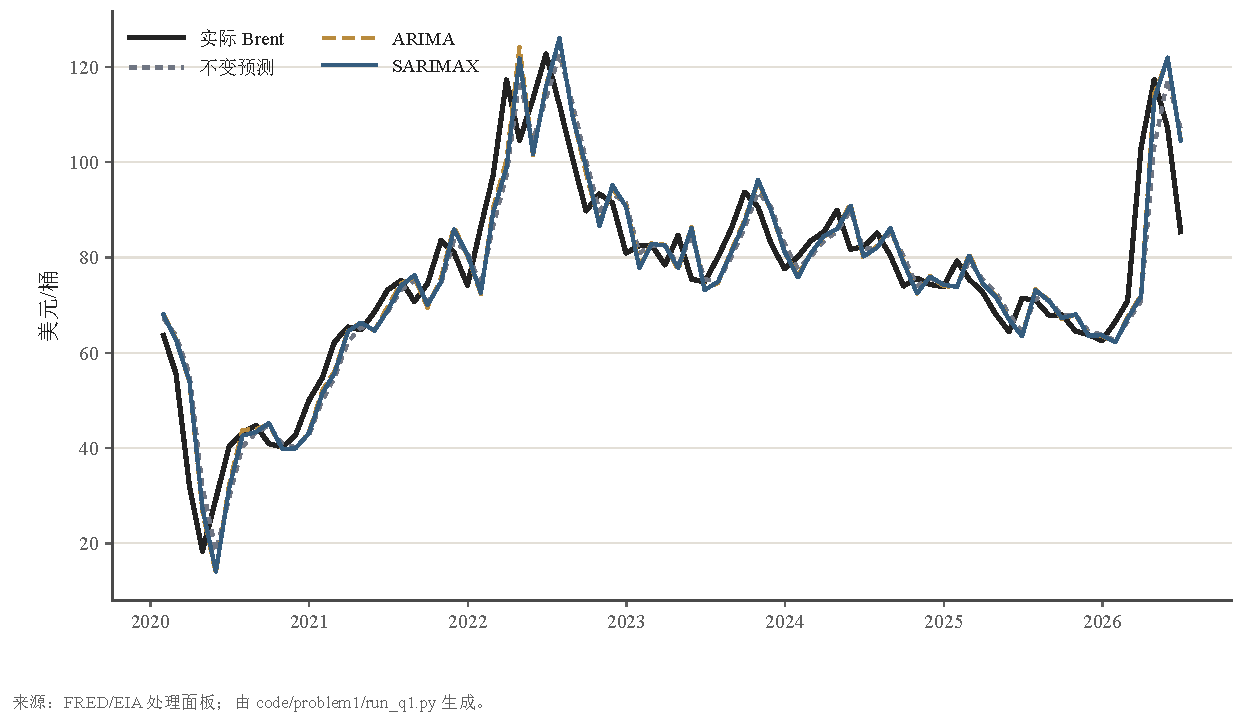
\includegraphics[width=0.90\textwidth]{../figures/q1_forecast_1m.pdf}
  \caption{Brent一月期扩展窗口预测与实际值}
  \label{fig:q1-forecast}
\end{figure}

\subsection{多阶段事件研究}

冲突日期与政策日期按表\ref{tab:event-timeline}分开编码。对2024年1月至事件前最后
交易日的Brent日收益拟合AR(3) 并控制广义美元收益，得到条件期望
$\widehat r_t^{,0}$。异常收益及累计异常收益定义为

\begin{equation}
  AR_t=r_t-\widehat r_t^{\,0},\qquad
  CAR[0,H]=\sum_{j=0}^{H}AR_{t_0+j},\quad H=0,1,2.
  \label{eq:car}
\end{equation}

为避免把单日常规标准误当作强因果证据，本文从非事件周末构造同口径伪事件。若 $B$
个安慰剂窗口中有 $b$ 个绝对CAR不小于真实事件，则经验显著性采用
$p_{emp}=(b+1)/(B+1)$，从而不会报告有限样本下不合理的零概率。

\begin{table}[H]
  \centering
  \small
  \caption{外部冲突、航运受阻、国内调控与缓和阶段时间线}
  \label{tab:event-timeline}
  \begin{tabularx}{0.97\textwidth}{p{0.13\textwidth}p{0.13\textwidth}p{0.20\textwidth}Xp{0.13\textwidth}}
    \toprule
    日期 & 编号 & 事件 & 主要通道 & 模型用途 \\
    \midrule
    2026-02-28 & E1 & 军事行动开始 & 供给中断风险、预防性需求与风险溢价 & 事件起点 \\
    2026-03-02 & E2 & 海峡运输受阻 & 实物流量、运价与保险成本 & 阶段变量 \\
    2026-03-23、04-07 & P1、P2 & 中国临时调控 & 降低当期国内价格传导 & 政策反事实 \\
    2026-06-17 & E3 & 通行恢复谅解 & 供应恢复预期与风险溢价回落 & 缓和阶段 \\
    \bottomrule
  \end{tabularx}
\end{table}

\begin{table}[H]
  \centering
  \small
  \caption{E1事件窗口的Brent累计异常收益}
  \label{tab:q1-car}
  \begin{tabular}{ccccc}
    \toprule
    窗口 & CAR & 常规95\% 区间 & 经验 $p$ 值 & 交易日数 \\
    \midrule
    $[0]$ & 0.0797 & $[0.0415,\,0.1178]$ & 0.0112 & 1 \\
    $[0,+1]$ & 0.1561 & $[0.1021,\,0.2101]$ & 0.0102 & 2 \\
    $[0,+2]$ & 0.1355 & $[0.0694,\,0.2016]$ & 0.0208 & 3 \\
    \bottomrule
  \end{tabular}
\end{table}

三组CAR均高于绝大多数匹配周末安慰剂，说明E1附近存在经济量级较大的事件相关
异常上涨。与此同时，战前模型递归生成的价格路径与实际价格之差记作

\begin{equation}
  ARBaselineGap_t=P_t-\widehat P_t^{\,AR\ baseline}.
  \label{eq:argap}
\end{equation}

该差额用于展示实际走势偏离战前自回归规律的程度；由于同期供需和其他新闻不能完全
排除，本文不将其称为``无战争价格''或战争净溢价。

\subsection{结构冲击与条件波动}

为给第二问提供具有经济含义的月度冲击，构造向量
$z_t=(\Delta q_t,a_t,\Delta p_t^{real})^{\mathsf T}$，分别表示全球液体燃料供给增长、
全球真实活动和实际Brent收益，并估计

\begin{equation}
  A(L)z_t=u_t,\qquad u_t=B\epsilon_t,
  \label{eq:svar}
\end{equation}

其中 $B$ 由Cholesky分解识别。BIC选出6阶稳定VAR，白噪声检验
$p=0.382$，三类结构冲击均有186个有效月。该分解遵循不同油价冲击不能混为一谈的
原则\cite{kilian2009}，但仍受递归排序约束。

日度波动采用战前样本拟合GJR--GARCH(1,1)：

\begin{equation}
  h_t=\omega+\alpha\varepsilon_{t-1}^{2}
  +\gamma I(\varepsilon_{t-1}<0)\varepsilon_{t-1}^{2}+\beta h_{t-1}.
  \label{eq:gjr}
\end{equation}

战前条件波动率中位数为1.743\%。E1即时窗口、E2航运受阻阶段和E3缓和阶段分别为
战前的1.587、2.214和1.566倍。可见波动压力在事实性运输受阻阶段最高，缓和后虽有
下降但尚未回到战前水平。该结果只描述金融市场波动，不能直接解释为实体经济损失。

\subsection{问题一小结}

预测层面，no-change在固定回测中诚实胜出；事件层面，E1三个交易日窗口的CAR及
安慰剂检验支持显著的事件相关异常上涨；机制层面，递归VAR输出供给、需求和石油特定
风险冲击，GJR--GARCH则显示航运受阻阶段条件波动最强。三类证据共同回答题意，但不把
预测误差、描述性基准差额或单次事件关联夸大为战争的严格净因果贡献。

\section{问题二：油价冲击对中国经济的传导}

\subsection{变量特定的局部投影}

人民币原油成本构造为

\begin{equation}
  C_t^{oil}=P_t^{Brent,USD}FX_t^{CNY/USD},\qquad
  c_t=100\Delta\ln C_t^{oil}.
  \label{eq:oilcost}
\end{equation}

结构冲击的来源不同，其宏观含义也不同\cite{tang2010,cross2017,chen2020}。本文分别输入
不利供给、全球需求和石油特定风险冲击；未分解$OilShock$只作约化形式稳健性。局部投影不对整条
脉冲路径施加强递推限制\cite{jorda2005}，但被解释变量必须与程序定义一致。对PPI、CPI、IAV和
人民币原油成本，估计未来水平响应

\begin{equation}
  y_{t+h}=\alpha_h+\theta_hs_t+\rho_hy_{t-1}+\eta_hs_{t-1}
  +\Gamma_h^{\mathsf T}Z_{t-1}+u_{t+h};
  \label{eq:lp-level}
\end{equation}

对汇率则估计相对冲击前基期的累计变化

\begin{equation}
  100(\ln FX_{t+h}-\ln FX_{t-1})
  =\alpha_h+\theta_hs_t+\rho_h\Delta\ln FX_{t-1}
  +\eta_hs_{t-1}+\Gamma_h^{\mathsf T}Z_{t-1}+u_{t+h}.
  \label{eq:lp-fx}
\end{equation}

$Z_{t-1}$包含美元、GPR、月份虚拟变量和疫情阶段。PPI、CPI、成本和汇率估计$h=0,\ldots,12$；
IAV因1至2月结构性缺失，只估计$h\in\{0,3,6,12\}$。使用同源移动块bootstrap和最大$t$统计量
构造95\%联合置信带。对完整月度路径定义响应曲线面积

\begin{equation}
  A_y(H)=\sum_{h=0}^{H}\widehat\theta_{y,h},
  \label{eq:response-area}
\end{equation}

单位为“百分点月”，只描述离散响应曲线的面积，不称为累计经济损失。IAV的四个稀疏期限不求和。

\begin{figure}[htbp]
  \centering
  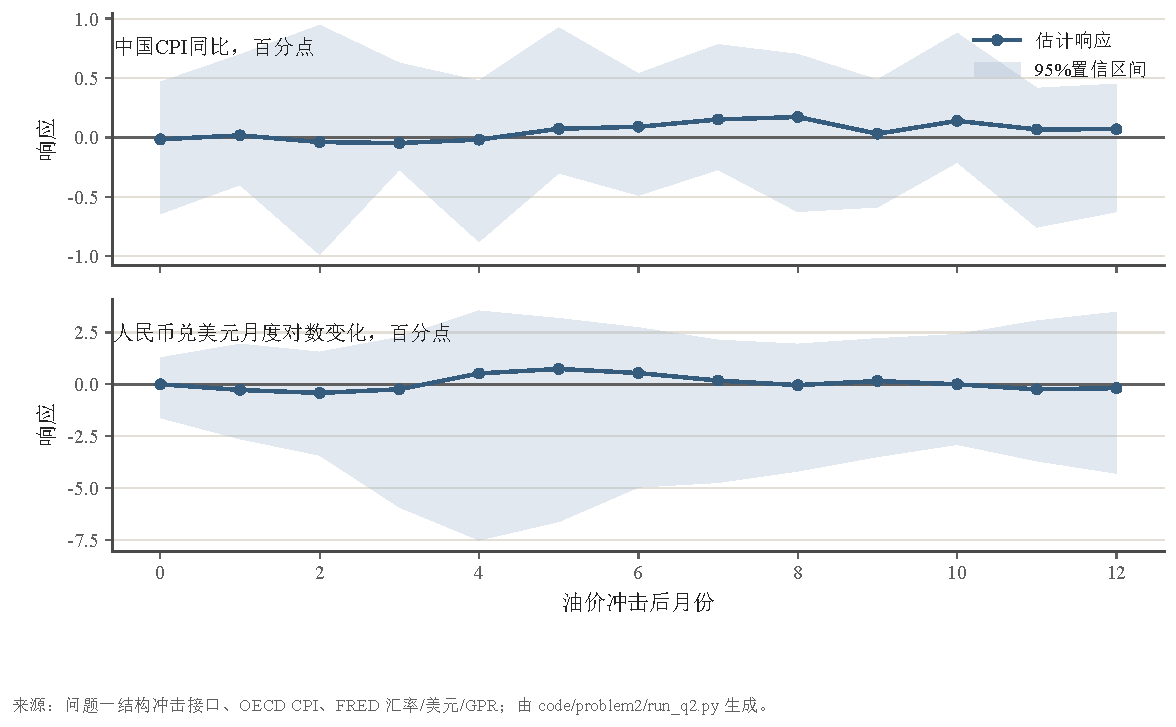
\includegraphics[width=0.91\textwidth]{../figures/q2_irf.pdf}
  \caption{油价特定风险冲击下中国主要变量的局部投影响应}
  \label{fig:q2-irf}
\end{figure}

\subsection{油价特定风险冲击结果}

\begin{table}[htbp]
  \centering
  \small
  \caption{油价特定风险冲击的传导指标}
  \label{tab:q2-metrics}
  \begin{tabularx}{0.98\textwidth}{Xccccc}
    \toprule
    结果变量 & 极值 & 月份 & 极值联合95\%区间 & $A(0,6)$ & $A(0,12)$ \\
    \midrule
    人民币原油成本 & 8.832 & 0 & $[6.888,10.776]$ & 7.440 & 4.939 \\
    PPI同比 & 0.762 & 10 & $[-0.159,1.684]$ & 3.655 & 7.401 \\
    CPI同比 & 0.247 & 7 & $[-0.096,0.589]$ & 0.877 & 2.155 \\
    IAV同比 & $-0.427$ & 12 & $[-0.966,0.111]$ & -- & -- \\
    人民币汇率 & 0.771 & 12 & $[-0.488,2.030]$ & 1.612 & 5.846 \\
    \bottomrule
  \end{tabularx}
\end{table}

成本入口当月响应最清晰；PPI和CPI点估计滞后上行，IAV在12个月出现负向点估计。但除成本入口外，
极值的联合区间均跨零，故不能将点估计写成稳健总体增长损失。季度GDP在加入所需滞后后没有足够
有效观测，低频验证状态为“结论不充分”，也不再报告旧版小样本回归值。

不同结构冲击的响应方向并不相同：全球需求扩张可同时推高油价和产出，不利供给或石油特定风险
更符合成本推动机制。这解释了为何“油价上涨”不能直接等同于“经济受损”。ARDL、疫情剔除、
冲击正负拆分和替代排序只作为稳健性探针；它们未把工业活动和GDP证据提升为联合显著。

\subsection{问题二小结}

模型支持“进口成本快速响应、PPI和CPI滞后上行、工业活动可能承压”的传导顺序，但总体增长损失
仍为结论不充分。后续政策评价必须同时报告物价、工业活动、响应期限和区间，不能只比较单一价格
传导系数。

\section{问题三：中国政策缓冲与跨国比较}

\subsection{先锁定可比边界}

跨国燃油传导受税制、汇率和定价机制共同影响\cite{kpodar2017,kpodar2021}。对每个国家估计

\begin{equation}
  \Delta\ln F_{i,t}=a_i+\varphi_i\Delta\ln F_{i,t-1}
  +\sum_{j=0}^{6}\beta_{i,j}\Delta\ln P^{Brent,local}_{i,t-j}+u_{i,t},
  \label{eq:fuel-dl}
\end{equation}

并以$\Pi_{i,H}=\sum_{j=0}^{H}\beta_{i,j}$表示$H$月传导率。德国、法国、意大利、西班牙、日本
和韩国有可审计的固定品类零售燃油价格，进入正式排名。中国历史公开调价表只能重建出受管制汽油
调价指数代理，不是固定标准品零售价格，因此从正式排名剔除，只保留为敏感性和政策路径构造。

\begin{figure}[htbp]
  \centering
  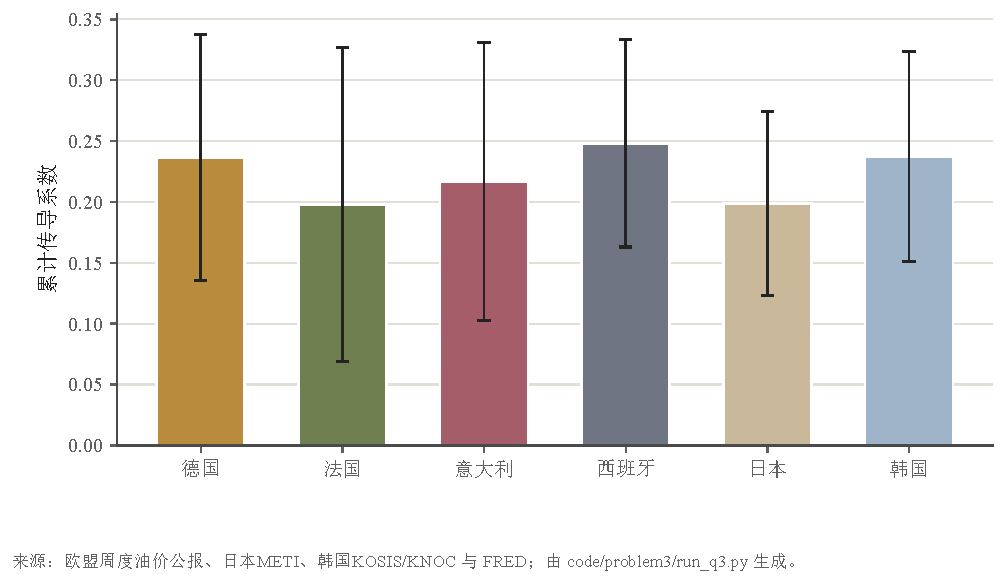
\includegraphics[width=0.91\textwidth]{../figures/q3_pass_through_6m.pdf}
  \caption{六国正式零售价格与中国调价指数代理的六个月传导率}
  \label{fig:q3-pass}
\end{figure}

\begin{table}[htbp]
  \centering
  \small
  \caption{六个月燃油传导率及数据角色}
  \label{tab:q3-pass}
  \begin{tabular}{lccccccc}
    \toprule
    国家 & 中国 & 德国 & 法国 & 意大利 & 西班牙 & 日本 & 韩国 \\
    \midrule
    传导率 & 0.373 & 0.237 & 0.198 & 0.217 & 0.248 & 0.199 & 0.237 \\
    数据角色 & 代理敏感性 & 正式 & 正式 & 正式 & 正式 & 正式 & 正式 \\
    \bottomrule
  \end{tabular}
\end{table}

六个正式对照国中位数为0.227。中国代理值0.373较高，但二者并非同类价格层，故不能据此判断
中国更优或更差。这个“不可比”结论本身是重要的数据审计结果。

\subsection{代理排名的临界误差与部分识别}

为了把“不可比”从定性提醒改成可检验边界，定义中国真实固定品类零售价格传导率与调价指数代理
之间的缩放关系

\begin{equation}
  \Pi_{\mathrm{CN,true}}=\kappa \Pi_{\mathrm{CN,proxy}}.
  \label{eq:q3-kappa}
\end{equation}

以六国中位数0.227和中国代理值0.373计算，临界缩放系数为
$\kappa^\ast=0.227/0.373=0.607$。这意味着：只有当真实固定品类零售价的六个月传导约低于
调价指数代理变化的61\%时，中国才可能落到六国中位数以下。长度为6个月的时间块bootstrap给出
均匀缩放情形下$\kappa^\ast$中位数0.590，95\%区间为$[0.436,0.834]$；前置折价与后置折价扰动
下区间分别为$[0.461,0.849]$和$[0.578,1.169]$。因此该计算只能量化代理误差需要多大，不能
把中国重新放回正式国别排名。

\begin{figure}[htbp]
  \centering
  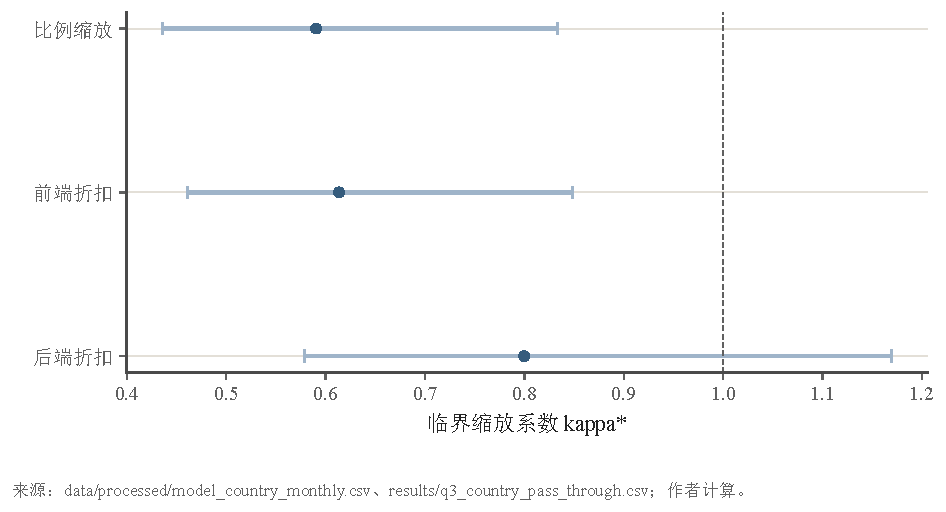
\includegraphics[width=0.72\textwidth]{../figures/paper_extension_q3_partial_identification.pdf}
  \caption{中国代理传导率进入正式排名所需的临界缩放系数}
  \label{fig:q3-partial-identification}
\end{figure}

\subsection{相对宏观响应与暂缓的机制回归}

对CPI和工业活动估计含国家固定效应和完整年月固定效应的面板局部投影：

\begin{equation}
  y_{i,t+h}-y_{i,t-1}=\alpha_{i,h}+\lambda_{t,h}
  +\delta_{i,h}(s_tI_i)+\Gamma_h^{\mathsf T}Z_{i,t-1}+u_{i,t+h}.
  \label{eq:panel-lp}
\end{equation}

中国是参照组，$\delta_{i,h}$只表示对照国相对中国的响应差，不能把中国绝对响应人为设为零。
对照国减中国的CPI相对响应点估计中位数为0.245个百分点，工业活动为2.433个百分点；但当前
程序没有形成联合国别--时间bootstrap区间，因此两项均判为“结论不充分”。价格监管、进口依赖、
石油强度和进口来源集中度年度表均为未经审计代理，四类连续缓冲交互回归全部执行失败关闭，不提供
系数、显著性或政策排序。三维核心韧性判据见表\ref{tab:q3-resilience}。

\begin{table}[htbp]
  \centering
  \small
  \caption{中国相对韧性的核心判据}
  \label{tab:q3-resilience}
  \begin{tabularx}{0.96\textwidth}{p{0.23\textwidth}Xp{0.22\textwidth}}
    \toprule
    维度 & 当前证据 & 判断 \\
    \midrule
    燃油价格 & 中国仅有调价指数代理，不能与六国固定品类零售价正式排名 & 条件代理 \\
    消费价格 & 对照国减中国点估计中位数0.245，缺联合差异区间 & 结论不充分 \\
    工业活动 & 对照国减中国点估计中位数2.433，缺联合差异区间 & 结论不充分 \\
    \midrule
    总体 & 任一核心维度均不足以形成稳健“更好”判断 & 结论不充分 \\
    \bottomrule
  \end{tabularx}
\end{table}

\subsection{关闭2026年临时调控的动态反事实}

依据《石油价格管理办法》\cite{ndrc2016}和2026公告核验，3月汽油机制应调2205元/吨、实调
1160元/吨，新增缺口1045元/吨；4月机制应调800元/吨、实调420元/吨，新增380元/吨，累计
缺口1425元/吨。令$P_t^{no}$和$P_t^{act}$分别为无临时调控与实际代理价格路径，输入模型的不是
静态价格水平差，而是逐月收益差

\begin{equation}
  \Delta f_t=100\left[\ln\frac{P_t^{no}}{P_{t-1}^{no}}
  -\ln\frac{P_t^{act}}{P_{t-1}^{act}}\right].
  \label{eq:fuel-return-gap}
\end{equation}

对$y\in\{PPI,CPI,IAV\}$，用0至6阶动态核和结果变量AR(1)递推：

\begin{equation}
  B_{y,t}=\sum_{\ell=0}^{6}\beta_{y,\ell}\Delta f_{t-\ell}
  +\phi_yB_{y,t-1}.
  \label{eq:policy-dynamic}
\end{equation}

三条方程使用同一组长度为6的循环时间块联合抽样，共接受2000组参数抽样，从而保留PPI、CPI和
IAV估计误差的同期相关。

\begin{figure}[htbp]
  \centering
  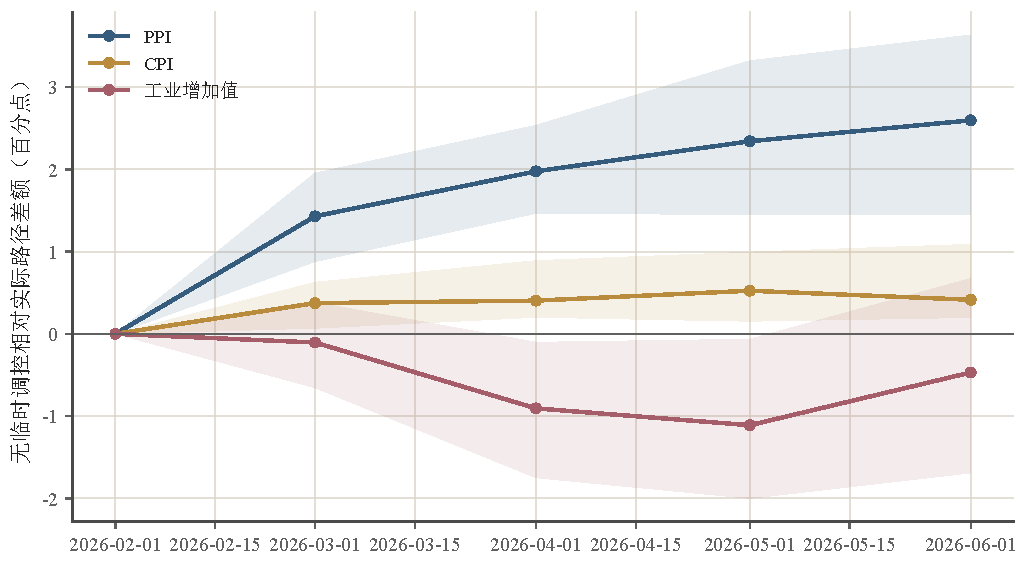
\includegraphics[width=0.91\textwidth]{../figures/q3_policy_macro_counterfactual.pdf}
  \caption{关闭临时调控后的动态宏观情景差额}
  \label{fig:q3-policy-macro}
\end{figure}

\begin{table}[htbp]
  \centering
  \small
  \caption{2026年6月无临时调控减实际路径的宏观差额}
  \label{tab:q3-policy}
  \begin{tabular}{lccc}
    \toprule
    变量 & 情景差额/百分点 & 95\%区间 & 情景证据 \\
    \midrule
    PPI & 2.596 & $[1.453,3.633]$ & 区间不跨零 \\
    CPI & 0.414 & $[0.199,1.088]$ & 区间不跨零 \\
    IAV & $-0.469$ & $[-1.690,0.672]$ & 结论不充分 \\
    \bottomrule
  \end{tabular}
\end{table}

结果说明，在维持动态核与局部环境不变的条件下，临时调控可能降低了2026年6月PPI和CPI压力；
IAV方向符合缓冲解释但区间跨零。该结论依赖调价指数代理，不能外推为全面福利改善，也不改变跨国
总体韧性“结论不充分”的判断。

\begin{table}[htbp]
  \centering
  \small
  \caption{政策工具、作用渠道与证据等级}
  \label{tab:q3-policy-evidence}
  \begin{tabularx}{0.98\textwidth}{p{0.18\textwidth}Xp{0.20\textwidth}p{0.20\textwidth}}
    \toprule
    政策工具 & 作用渠道 & 正文证据 & 证据边界 \\
    \midrule
    成品油价格监管 & 延缓原油成本向PPI和CPI传导，同时形成未调价缺口 & 2026年动态反事实；PPI、CPI区间不跨零 & 条件情景，不等于福利评估 \\
    进口来源多元化 & 降低单一区域供给中断暴露 & 机制解释与数据审计 & 连续HHI未审计，不估计交互系数 \\
    石油进口依赖度 & 决定国际价格冲击进入国内成本的暴露度 & 文献机制与国别描述 & 年度代理不足以支持月度因果结论 \\
    石油强度 & 决定单位产出的燃油和运输成本敏感性 & 文献机制与产业链解释 & 不恢复未审计缓冲回归 \\
    战略储备、汇率与财政措施 & 通过库存释放、汇率稳定和补贴减轻短期压力 & 作为边界条件讨论 & 缺连续、可比强度数据，不作量化排序 \\
    \bottomrule
  \end{tabularx}
\end{table}

\subsection{问题三小结}

正式零售价格、相对宏观响应和政策反事实属于三类不同证据。当前数据不能证明中国在三维韧性上
全面优于对照国；较强的结论只限于2026年条件情景中PPI与CPI的局部缓冲，同时必须显式记录
1425元/吨延期缺口及其后续消化责任。

\section{问题四：极端油价风险与自适应调价规则}

\subsection{条件尾部分布：FHS--GJR--GARCH}

前三问研究已实现冲击，问题四进一步回答：在2026年6月30日信息集下，未来油价
进入历史高位区间的条件概率多大，以及国内调价机制应如何随压力状态变化。令日收益率
$r_t=\mu+\varepsilon_t$，条件方差服从式\eqref{eq:gjr}。先估计GJR--GARCH，再将
标准化残差 $z_t=\varepsilon_t/\sqrt{h_t}$ 从截止日前经验分布有放回抽样，递归生成

\begin{equation}
  P_{t+k}^{(b)}=P_{t+k-1}^{(b)}
  \exp\!\left(\mu+\sqrt{h_{t+k}^{(b)}}z_{t+k}^{(b)}\right).
  \label{eq:fhs}
\end{equation}

每个期限模拟20000条路径。基线为恒定均值、恒定波动的高斯随机游走，并与主方法使用
相同滚动原点、期限和评价口径。历史90\% 与95\% 价格分位分别为111.397和
115.550美元/桶，只作为上行压力阈值，不作为未来必达价格。

\begin{figure}[H]
  \centering
  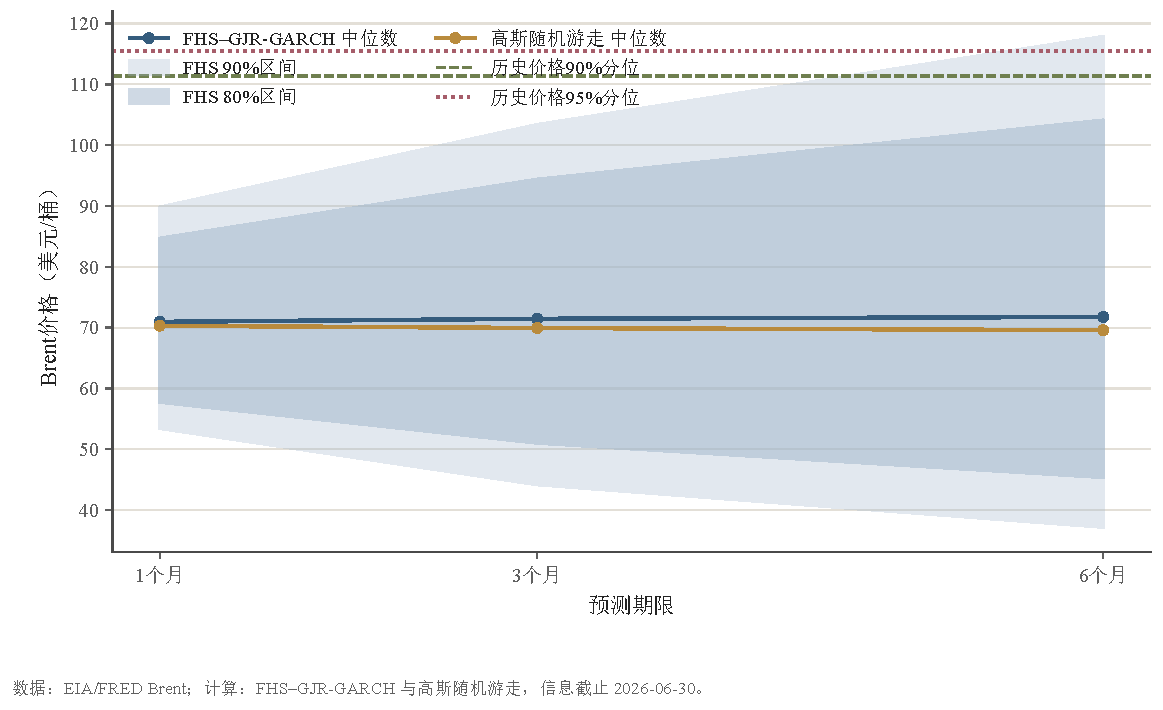
\includegraphics[width=0.91\textwidth]{../figures/q4_price_tail_risk.pdf}
  \caption{固定截止日下Brent条件尾部分布与历史高位阈值}
  \label{fig:q4-tail}
\end{figure}

\begin{table}[H]
  \centering
  \small
  \caption{FHS--GJR--GARCH的油价条件风险预测}
  \label{tab:q4-tail}
  \begin{tabular}{ccccc}
    \toprule
    期限/月 & 中位数 & 90\% 区间 & 期末超过历史95\% 阈值 & 路径内曾越过 \\
    \midrule
    1 & 70.95 & $[53.41,\,89.82]$ & 0.27\% & 0.37\% \\
    3 & 71.46 & $[44.15,\,103.41]$ & 2.27\% & 3.76\% \\
    6 & 71.76 & $[37.15,\,117.90]$ & 5.56\% & 9.65\% \\
    \bottomrule
  \end{tabular}
\end{table}

随着期限延长，中位数仍约为71美元/桶，但分布显著展开，六个月路径内越过历史95\%
阈值的条件概率达到9.65\%。15个季度末原点的统一回测显示：FHS与高斯基线在1、3、
6月的平均分位损失分别为1.639对1.624、2.303对2.483、3.888对3.814。
主方法只在三月期损失更低，而其90\% 区间平均宽度在三个期限均较窄。因此，FHS的
价值主要在于刻画条件异方差和非对称尾部，并非所有期限都全面胜过简单基线。

\subsection{结构冲击宏观压力与已实现政策缓冲}

为避免把模拟价格机械转换为结构冲击，宏观压力直接使用问题一石油特定风险冲击的历史
正向75\%、90\%、95\% 分位数 $s_q$，按

\begin{equation}
  \Delta y_h(s_q)=s_q\widehat\theta_{y,h}
  \label{eq:macrostress}
\end{equation}

缩放问题二响应及联合置信区间。95\% 分位冲击值为1.471。其6月和12月条件响应中，
PPI为0.875、0.493个百分点，CPI为0.267、0.240个百分点，IAV为 $-0.435$、
$-0.628$ 个百分点；六项联合95\% 区间均跨零，故只作为条件压力情景。

政策压力层不把上述情景与问题三反事实相加，而只重述已实现2026路径：相对关闭临时
调控，实际政策截至6月避免的PPI、CPI上行分别为3.370和0.819个百分点，避免的
IAV损失为2.093个百分点。前者来自历史结构冲击的条件响应，后者来自已实现政策路径的
局部反事实，二者识别层级不同。

\subsection{SAPR--CVaR三状态调价规则}

固定传导率难以同时兼顾日常价格信号和极端期宏观稳定。本文在现行机制应调额
$A_t^{rule}$ 上增加状态自适应平滑层。用开发样本中正向机制应调额的75\% 和95\%
分位确定压力阈值435.973和702.491元/吨，并将月份划分为普通、压力和极端状态。
设相应传导率为 $\rho_N\ge\rho_S\ge\rho_E$。若上期仍有未调价差额 $G_{t-1}$，则

\begin{align}
  D_t &= A_t^{rule}+G_{t-1}, \\
  A_t^{SAPR} &=
  \begin{cases}
    \rho_{g_t}D_t, & D_t>0,\\
    D_t, & D_t\le 0,
  \end{cases} \\
  G_t &=
  \begin{cases}
    D_t-A_t^{SAPR}, & D_t>0,\\
    0, & D_t\le 0.
  \end{cases}
  \label{eq:sapr}
\end{align}

这里的负向应调额优先冲销延期差额，避免缺口无限积累。以2026年6月官方价格
9504元/吨为统一基价，将调价收益输入由问题三估计的PPI、CPI、IAV动态核。对每条
六个月情景计算标准化月度宏观损失

\begin{equation}
  L_s=\frac{1}{6}\sum_{t=1}^{6}\left[
  \frac{\max(PPI_{s,t},0)}{\sigma_{PPI}}+
  \frac{\max(CPI_{s,t},0)}{\sigma_{CPI}}+
  \frac{\max(-IAV_{s,t},0)}{\sigma_{IAV}}\right].
  \label{eq:macroloss}
\end{equation}

四个同时最小化的目标为

\begin{equation}
  J_1=\mathbb E(L_s),\quad
  J_2=CVaR_{0.95}(L_s),\quad
  J_3=\mathbb E\!\left[\frac{\sum_{t=1}^{6}G_{s,t}+G_{s,6}}{9504}\right],\quad
  J_4=SD(\Delta\ln F_{s,t}).
  \label{eq:objectives}
\end{equation}

传导率在 $\{0,0.05,\ldots,1\}$ 上枚举，并施加单调约束，共得到1771条规则。只使用
2013年3月至2021年12月的101个六个月开发情景选阈值和规则；2022年1月至
2026年6月的49个情景完全隔离用于检验。对四目标做Pareto支配筛选后保留855条
规则，再将各目标在Pareto集内归一化，选择到理想点欧氏距离最小的唯一膝点。

\begin{figure}[H]
  \centering
  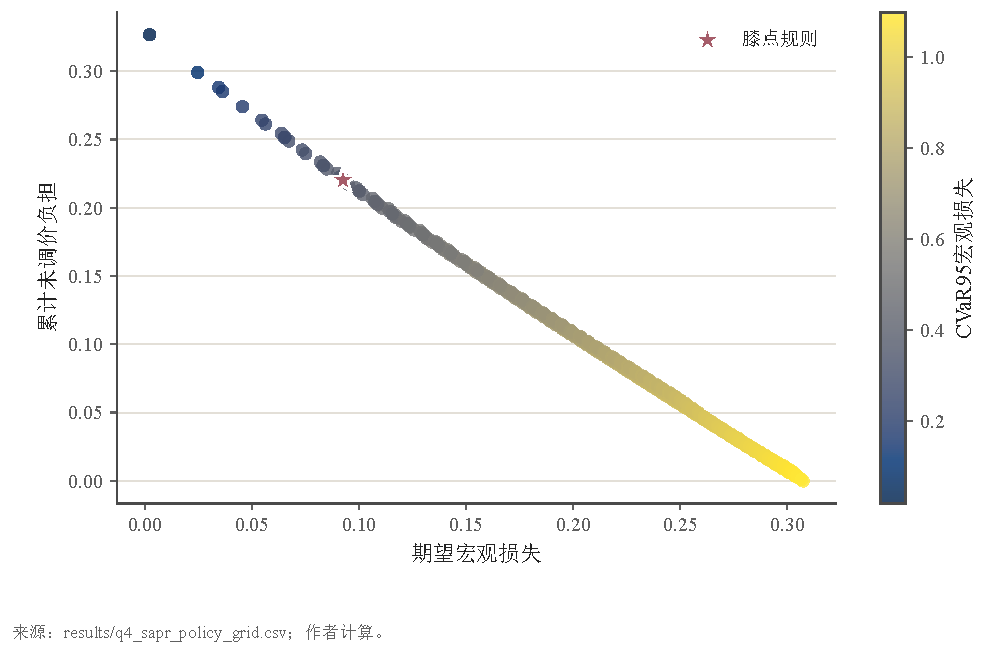
\includegraphics[width=0.88\textwidth]{../figures/q4_sapr_pareto_front.pdf}
  \caption{SAPR--CVaR四目标Pareto前沿与膝点规则}
  \label{fig:q4-pareto}
\end{figure}

膝点规则及其开发样本四目标分别为
\begin{equation}
  (\rho_N,\rho_S,\rho_E)=(0.20,0.05,0.05),
  \label{eq:sapr-knee}
\end{equation}
\begin{equation}
  (J_1,J_2,J_3,J_4)=(0.0925,0.3733,0.2201,0.0317).
  \label{eq:sapr-dev-objectives}
\end{equation}
隔离检验结果见表\ref{tab:q4-sapr}和图\ref{fig:q4-strategy}。

\begin{table}[H]
  \centering
  \small
  \caption{隔离检验样本的调价策略比较}
  \label{tab:q4-sapr}
  \begin{tabularx}{0.97\textwidth}{Xcccc}
    \toprule
    策略 & 平均宏观损失 $J_1$ & 95\% CVaR $J_2$ & 延期负担 $J_3$ & 调价波动 $J_4$ \\
    \midrule
    SAPR膝点 & 0.0908 & 0.5580 & 0.2394 & 0.0255 \\
    完全传导 & 0.3155 & 1.9571 & 0 & 0.0503 \\
    2026临时调控近似 & 0.2941 & 1.7681 & 0.0221 & 0.0426 \\
    统一75\% 平滑 & 0.2812 & 1.7916 & 0.0370 & 0.0438 \\
    \bottomrule
  \end{tabularx}
\end{table}

\begin{figure}[H]
  \centering
  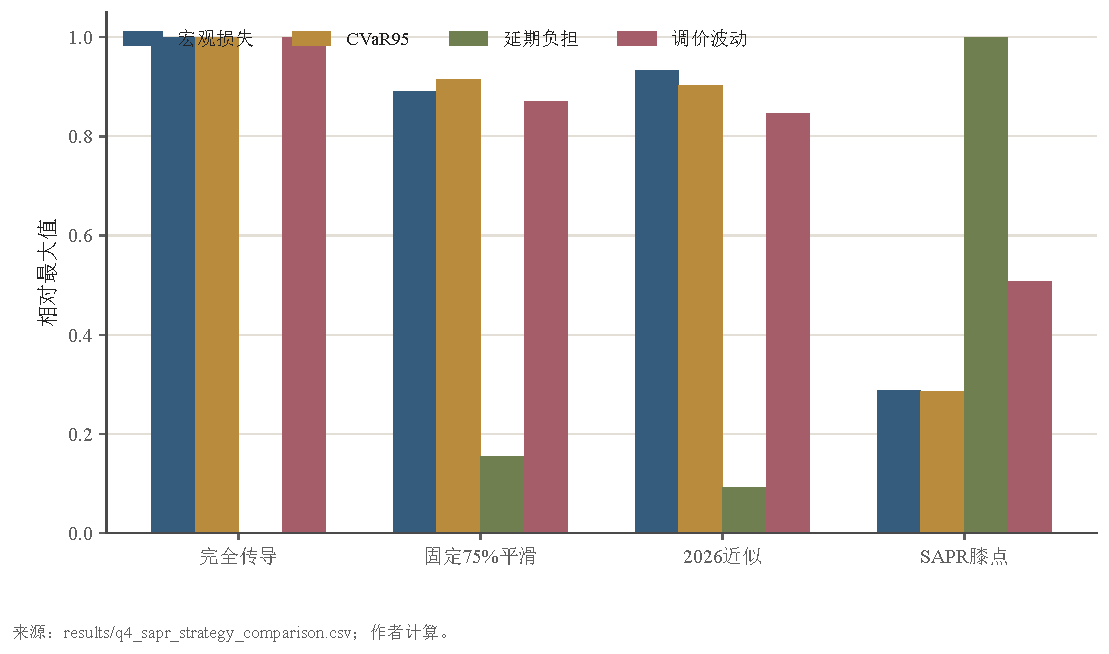
\includegraphics[width=0.90\textwidth]{../figures/q4_sapr_strategy_comparison.pdf}
  \caption{隔离检验样本中四类调价策略的多目标比较}
  \label{fig:q4-strategy}
\end{figure}

SAPR在检验样本的平均和尾部宏观损失、调价波动均低于三类预注册基线，但以较高延期
负担为代价。2000次参数抽样和块bootstrap中，SAPR保持不被基线支配的比例为1.000；
这表示模型参数不确定性下的相对稳定性，不是现实政策成功概率。2026实际冲击情景中，
SAPR、实际政策路径与完全传导的宏观损失分别为0.794、1.648和2.413，但SAPR延期
负担比例达到1.444，明显高于实际路径0.710。这一权衡说明极端期可以强化平滑，却必须
配套透明的缺口上限与退出机制。

\subsection{问题四小结}

固定截止日下，未来六个月Brent期末超过历史95\% 高位的条件概率为5.56\%，路径内
曾越过的概率为9.65\%；这些是风险分布而非确定预测。SAPR--CVaR在注册规则族内给出
普通期20\%、压力与极端期5\% 的膝点传导率，并在隔离检验中保持非支配，但延期负担
不可忽略。因此，建议把状态自适应平滑理解为临时风险管理层，而非替代现行定价机制的
无成本全局最优政策。

\section{稳健性与敏感性分析}

\subsection{预测、识别与传导探针}

问题一将六类预测器置于78个相同目标月比较；no-change在三个期限均取得最低RMSE，Theta虽接近，
DM--HLN检验未显示稳定优势。事件CAR改用40个前期波动率、价格水平和GPR状态最接近的安慰剂，
最小可实现经验$p$值为$1/41=0.0244$，避免普通周末样本造成虚假精度。结构VAR的6、12、18、
24阶候选均检查稳定性；6阶模型白噪声检验通过，替代排序下关键价格冲击相关系数不低于0.999。

问题二使用联合最大$t$置信带、逐点区间、FDR校正、ARDL、疫情剔除和冲击正负拆分。多数PPI、
CPI和IAV联合区间跨零，GDP有效观测不足，因此稳健性分析的作用是限制结论强度，而不是事后挑选
显著规格。问题三的四个年度缓冲变量因未经审计统一判为“主分析失败”，不以替代规格恢复定量结论。

\subsection{尾部风险回测}

FHS与高斯随机游走使用相同的47个月度原点和1、3、6个月期限。除分位损失和覆盖率外，补充80\%、
90\%区间分数与近似CRPS\cite{gneiting2007}。长度6的配对块bootstrap显示：FHS仅在3个月两档区间分数和6个月80\%
区间分数上显著更优，其余差异为结论不充分。由此将“FHS全面优于基线”列为禁止表述。

\subsection{SAPR规则敏感性}

\begin{table}[htbp]
  \centering
  \small
  \caption{SAPR膝点对阈值、权重和块长度的敏感性}
  \label{tab:q4-sensitivity}
  \begin{tabular}{lcccc}
    \toprule
    变体 & $(\rho_N,\rho_S,\rho_E)$ & Pareto数 & 相对默认变化 & 检验期非支配 \\
    \midrule
    默认75/95阈值 & $(0.30,0.10,0.10)$ & 119 & 否 & 是 \\
    70/90阈值 & $(0.30,0.15,0.10)$ & 82 & 是 & 是 \\
    80/97.5阈值 & $(0.30,0.10,0.10)$ & 209 & 否 & 是 \\
    CPI权重增加20\% & $(0.30,0.10,0.10)$ & 121 & 否 & 是 \\
    IAV权重增加20\% & $(0.30,0.10,0.10)$ & 116 & 否 & 是 \\
    bootstrap块3/6/12 & $(0.30,0.10,0.10)$ & 119 & 否 & 是 \\
    \bottomrule
  \end{tabular}
\end{table}

除较低状态阈值外，膝点规则对权重、阈值上界和块长度保持不变；70/90阈值把压力期传导率提高到
0.15，说明普通与压力状态的划分是最敏感设计项。所有变体在检验期点估计上保持非支配，但正文的
“支持”判断还依赖配对目标差和硬约束，而不只依赖非支配概率。

\section{模型评价与推广}

\subsection{模型优点}

\draftnote{从任务分层、可解释性、统一评价和可复现性四方面总结，避免“模型精度高”
等无证据套话。}

\subsection{模型局限}

\draftnote{讨论事件同期混杂、结构识别依赖、宏观样本长度、跨国价格口径和政策内生性。
每项局限对应一个可执行的改进方向。}

\subsection{推广方向}

\draftnote{说明框架如何推广到天然气、粮食或其他地缘风险驱动的大宗商品。}

\section{结论与政策启示}

\draftnote{按照四个问题依次给出结论，每条包含“方法--数值结果--现实含义”。政策建议
必须由模型结果支持，并区分短期价格平滑、中期供应安全和长期能源替代。}


\section*{AI工具使用说明}

本文在公开数据检索提示、程序调试、结果一致性检查和文字修改环节使用了OpenAI Codex。研究问题定义、模型取舍、数据口径、结果核验和最终表述均由参赛队独立判断并
承担责任；详细交互用途、采纳与人工修改情况见支撑材料《AI工具使用详情》。


\begin{thebibliography}{99}

\bibitem{kilian2009}
Kilian L. Not All Oil Price Shocks Are Alike: Disentangling Demand and Supply
Shocks in the Crude Oil Market[J]. American Economic Review, 2009, 99(3):
1053--1069. DOI: 10.1257/aer.99.3.1053.

\bibitem{caldara2022}
Caldara D, Iacoviello M. Measuring Geopolitical Risk[J]. American Economic
Review, 2022, 112(4): 1194--1225. DOI: 10.1257/aer.20191823.

\bibitem{baumeister2012}
Baumeister C, Kilian L. Real-Time Forecasts of the Real Price of Oil[J].
Journal of Business \& Economic Statistics, 2012, 30(2): 326--336.
DOI: 10.1080/07350015.2011.648859.

\bibitem{baumeister2015}
Baumeister C, Kilian L. Forecasting the Real Price of Oil in a Changing World:
A Forecast Combination Approach[J]. Journal of Business \& Economic Statistics,
2015, 33(3): 338--351. DOI: 10.1080/07350015.2014.949342.

\bibitem{jorda2005}
Jord\`a \`O. Estimation and Inference of Impulse Responses by Local
Projections[J]. American Economic Review, 2005, 95(1): 161--182.
DOI: 10.1257/0002828053828518.

\bibitem{diebold1995}
Diebold F X, Mariano R S. Comparing Predictive Accuracy[J]. Journal of
Business \& Economic Statistics, 1995, 13(3): 253--263.
DOI: 10.1080/07350015.1995.10524599.

\bibitem{harvey1997}
Harvey D, Leybourne S, Newbold P. Testing the Equality of Prediction Mean
Squared Errors[J]. International Journal of Forecasting, 1997, 13(2):
281--291. DOI: 10.1016/S0169-2070(96)00719-4.

\bibitem{glosten1993}
Glosten L R, Jagannathan R, Runkle D E. On the Relation between the Expected
Value and the Volatility of the Nominal Excess Return on Stocks[J]. Journal of
Finance, 1993, 48(5): 1779--1801.
DOI: 10.1111/j.1540-6261.1993.tb05128.x.

\bibitem{tang2010}
Tang W, Wu L, Zhang Z X. Oil Price Shocks and Their Short- and Long-Term
Effects on the Chinese Economy[J]. Energy Economics, 2010, 32(S1): S3--S14.
DOI: 10.1016/j.eneco.2010.01.002.

\bibitem{cross2017}
Cross J, Nguyen B H. The Relationship between Global Oil Price Shocks and
China's Output: A Time-Varying Analysis[J]. Energy Economics, 2017, 62:
79--91. DOI: 10.1016/j.eneco.2016.12.014.

\bibitem{chen2020}
Chen J, Zhu X, Li H. The Pass-Through Effects of Oil Price Shocks on China's
Inflation: A Time-Varying Analysis[J]. Energy Economics, 2020, 86: 104695.
DOI: 10.1016/j.eneco.2020.104695.

\bibitem{kpodar2017}
Kpodar K, Abdallah C. Dynamic Fuel Price Pass-Through: Evidence from a New
Global Retail Fuel Price Database[J]. Energy Economics, 2017, 66: 303--312.
DOI: 10.1016/j.eneco.2017.06.017.

\bibitem{kpodar2021}
Kpodar K, Imam P A. To Pass (or Not to Pass) Through International Fuel Price
Changes to Domestic Fuel Prices in Developing Countries: What Are the
Drivers?[J]. Energy Policy, 2021, 149: 111999.
DOI: 10.1016/j.enpol.2020.111999.

\bibitem{coady2013}
Coady D, Arze del Granado J, Eyraud L, et al. Automatic Fuel Pricing
Mechanisms with Price Smoothing: Design, Implementation, and Fiscal
Implications[R]. IMF Technical Notes and Manuals, 2013.
DOI: 10.5089/9781475566949.005.

\bibitem{coady2018}
Coady D, Parry I W H, Shang B. Energy Price Reform: Lessons for
Policymakers[J]. Review of Environmental Economics and Policy, 2018, 12(2):
197--219. DOI: 10.1093/reep/rey004.

\bibitem{baroneadesi2002}
Barone-Adesi G, Giannopoulos K, Vosper L. Backtesting Derivative Portfolios
with Filtered Historical Simulation[J]. European Financial Management, 2002,
8(1): 31--58. DOI: 10.1111/1468-036X.00175.

\bibitem{rockafellar2000}
Rockafellar R T, Uryasev S. Optimization of Conditional Value-at-Risk[J].
Journal of Risk, 2000, 2(3): 21--41. DOI: 10.21314/JOR.2000.038.

\bibitem{gneiting2007}
Gneiting T, Raftery A E. Strictly Proper Scoring Rules, Prediction, and
Estimation[J]. Journal of the American Statistical Association, 2007,
102(477): 359--378. DOI: 10.1198/016214506000001437.

\bibitem{ndrc2016}
国家发展和改革委员会. 石油价格管理办法[EB/OL]. 2016.
\url{https://www.ndrc.gov.cn/xxgk/zcfb/tz/201601/W020190905506573420251.pdf}.

\bibitem{freddata}
Federal Reserve Bank of St. Louis. FRED: Brent Crude Oil Price and Exchange
Rate Series[DB/OL]. \url{https://fred.stlouisfed.org/}. 访问日期：2026-07-30.

\bibitem{eiadata}
U.S. Energy Information Administration. Petroleum and Other Liquids Data,
Weekly U.S. Commercial Crude Oil Stocks[DB/OL].
\url{https://www.eia.gov/petroleum/data.php}. 访问日期：2026-07-30.

\bibitem{nbsdata}
国家统计局. 国家数据：月度与季度宏观指标[DB/OL].
\url{https://data.stats.gov.cn/}. 访问日期：2026-07-31.

\bibitem{oecddata}
OECD. Data Explorer: Consumer Prices and Industrial Production[DB/OL].
\url{https://data-explorer.oecd.org/}. 访问日期：2026-07-30.

\end{thebibliography}


\clearpage
\begin{appendices}

\section{支撑材料列表}

\begin{longtable}{p{0.34\textwidth}p{0.56\textwidth}}
  \caption{论文支撑材料及用途}\label{tab:support-files}\\
  \toprule
  文件或目录 & 功能说明 \\
  \midrule
  \endfirsthead
  \toprule
  文件或目录 & 功能说明 \\
  \midrule
  \endhead
  \texttt{code/problem1/} & 问题一预测、事件研究、结构冲击和波动率代码 \\
  \texttt{code/problem2/} & 问题二中国宏观传导代码 \\
  \texttt{code/problem3/} & 问题三跨国比较和政策反事实代码 \\
  \texttt{code/problem4/} & 自拟拓展的尾部风险和压力测试代码 \\
  \texttt{data/processed/} & 清洗后的建模数据及字段说明 \\
  \texttt{results/} & 冻结数值、诊断、回测和稳健性结果 \\
  \texttt{figures/} & 正文引用的 PDF 矢量图及 PNG 预览 \\
  \bottomrule
\end{longtable}

\section{核心代码说明}

\draftnote{正式提交时按比赛要求放入完整、可运行代码。若代码过长，正文附录至少给出
文件索引、入口命令和关键函数；支撑材料压缩包中保留全部代码与数据说明。}

\end{appendices}


\end{document}
